%%%%%%%%%%%%%%%%%%%%%%%%%%%%%%%%%%%%%%
% 
% TODO:
% 1. Figure out a smoother way for the document to flow onto the next page.
% 3. Add more icon options 
% 4. Fix hacky left alignment on contact line
% 5. Remove Hacky fix for awkward extra vertical space
% 
%%%%%%%%%%%%%%%%%%%%%%%%%%%%%%%%%%%%%%
%
% CHANGELOG:
%
%%%%%%%%%%%%%%%%%%%%%%%%%%%%%%%%%%%%%%%
%
% Known Issues:
% 1. Overflows onto second page if any column's contents are more than the vertical limit.
%%%%%%%%%%%%%%%%%%%%%%%%%%%%%%%%%%%%%%
%%Icons:
%%Main: https://icons8.com/icons/carbon-copy
%%%%%%%%%%%%%%%%%%%%%%%%%%%%%%%%%%

\documentclass[]{plushcv}
\usepackage{fancyhdr}
\pagestyle{fancy}
\fancyhf{}
% \rhead{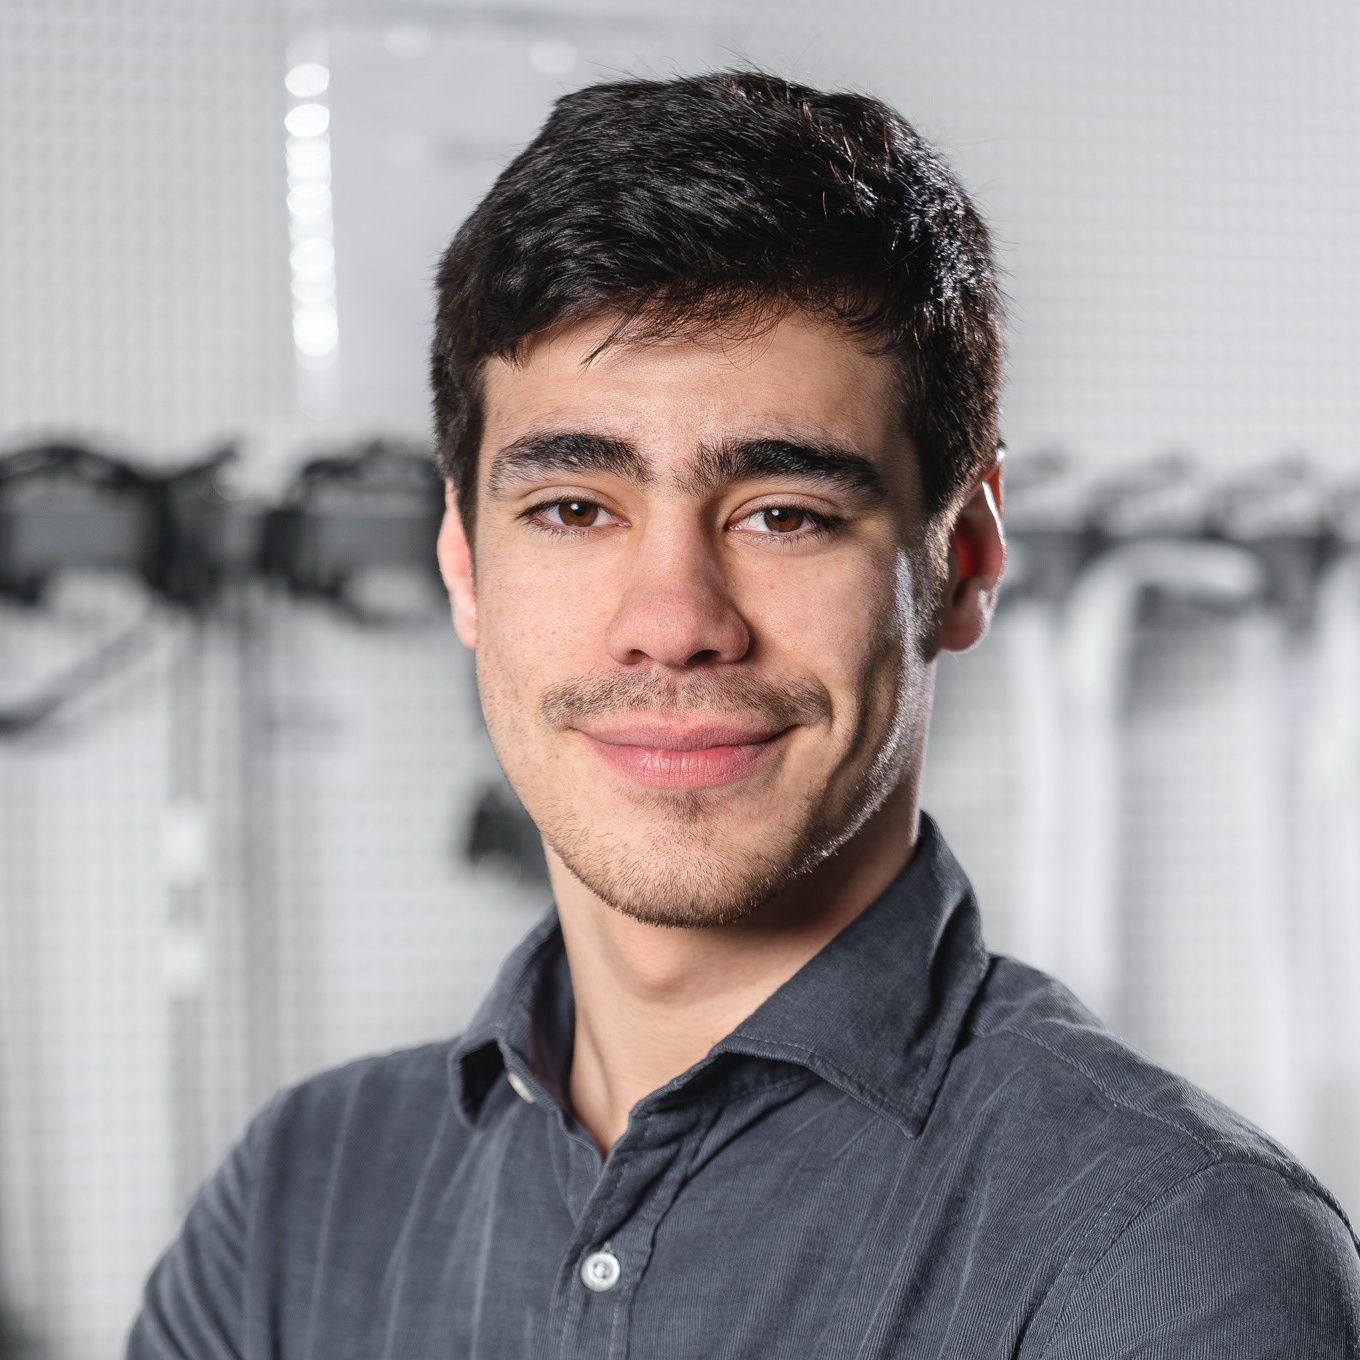
\includegraphics[width=5.5cm]{DMT.png}}
\begin{document}

%%%%%%%%%%%%%%%%%%%%%%%%%%%%%%%%%%%%%%
%
%     MY CV
%
%%%%%%%%%%%%%%%%%%%%%%%%%%%%%%%%%%%%%%

\namesection{David}{Munoz Tord}{}

{\contactline{\href{https://david-munoztord.com}{david-munoztord.com}}{\href{https://www.github.com/munoztd0}{munoztd0}}{\href{mailto:david.munoztord@mailbox.org}{david.munoztord@mailbox.org}}{\href{tel:+41792441756}{0792441756}}}
\hfill 
\smash{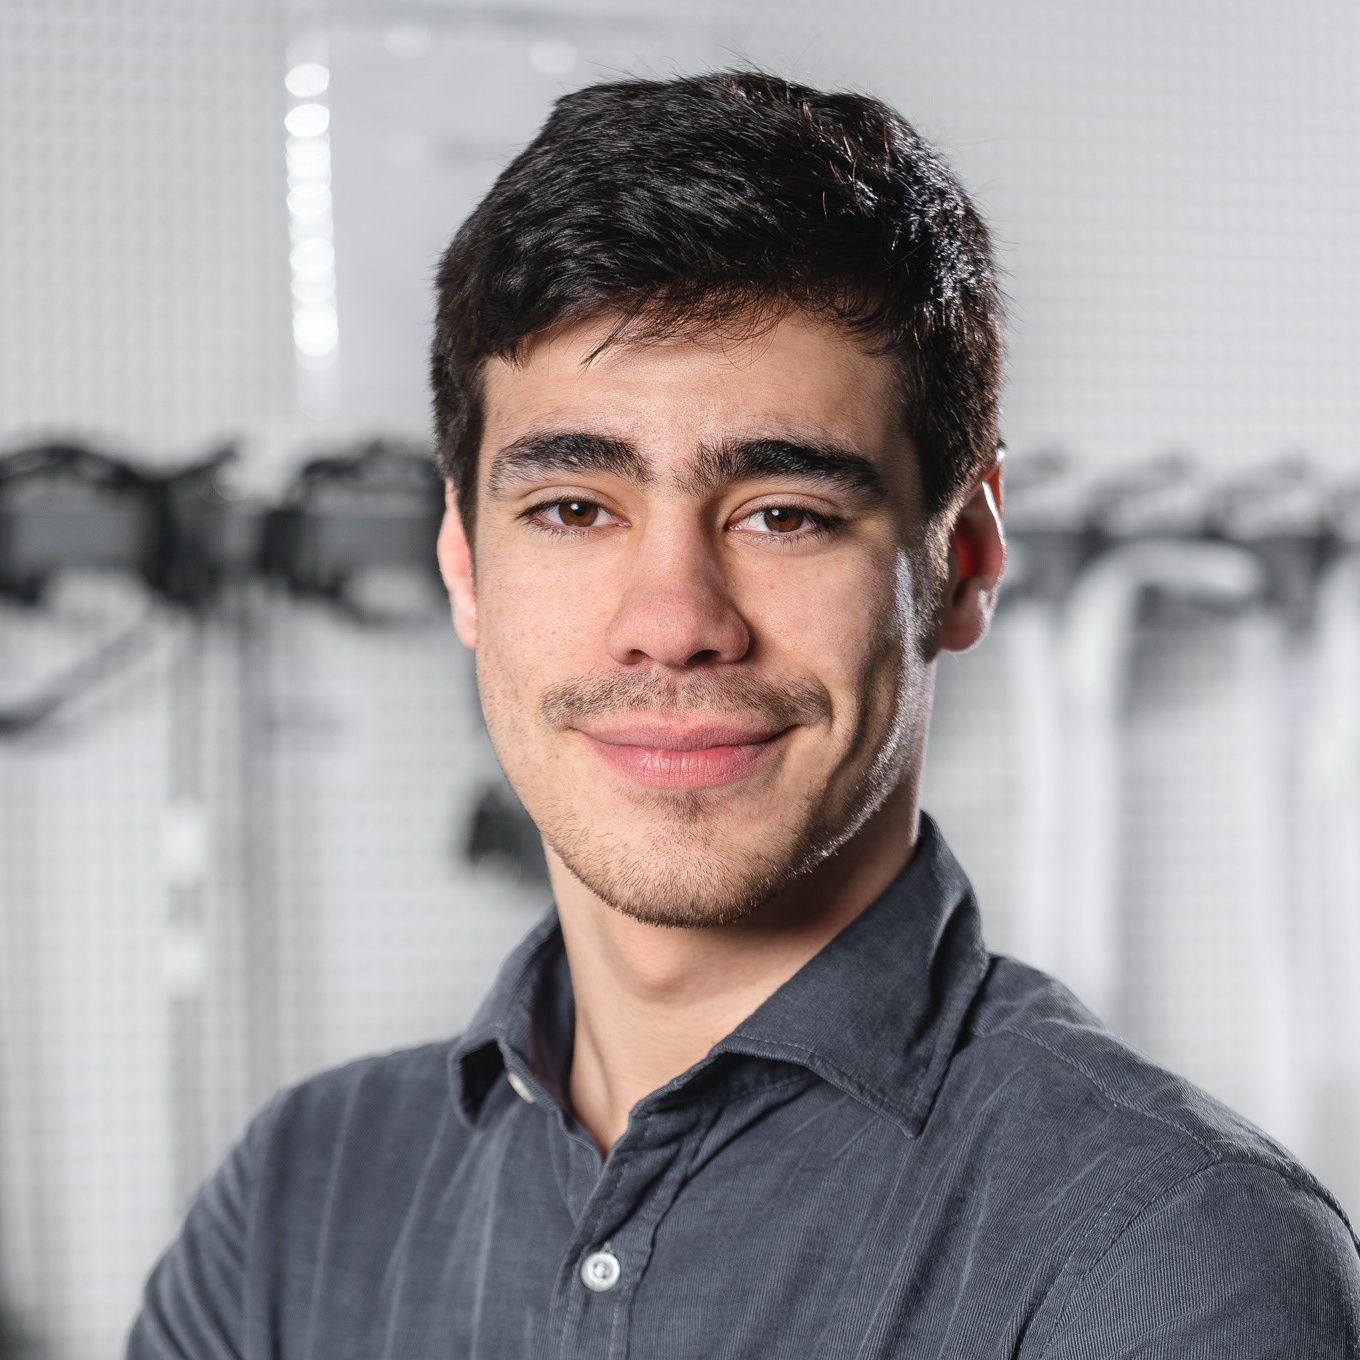
\includegraphics[width=3cm]{DMT.png}}
\sectionsep
\sectionsep
\sectionsep

%%%%%%%%%%%%%%%%%%%%%%%%%%%%%%%%%%%%%%
%
%     COLUMN ONE
%
%%%%%%%%%%%%%%%%%%%%%%%%%%%%%%%%%%%%%%

\begin{minipage}[t]{0.70\textwidth} 


%%%%%%%%%%%%%%%%%%%%%%%%%%%%%%%%%%%%%%
%     EXPERIENCE
%%%%%%%%%%%%%%%%%%%%%%%%%%%%%%%%%%%%%%
\sectionsep

\section{Experience}

\runsubsection{CICAD Organisation}
\descript{| Data Engineer }
\location{Part-time: October 2022 – Present | Geneva, Switzerland}
\begin{tightemize}
\sectionsep
\sectionsep
\item Worked closely with analysts across departments to design, build and deploy various initiatives within the data platform.
\item Developed, deployed and maintained data services using R and PostgreSQL.
\item Prepared and presented analysis for trimestrial reports.
\item Designed best practices to support continuous process automation for data ingestion and data pipeline workflows.
\item Automated amalgamation of data from spreadsheet revenue calculations and PDF reports reducing month end processing time from 2 days to 4 minutes.
\end{tightemize}
\sectionsep


\runsubsection{FlowBank SA}
\descript{| Data Engineer }
\location{Part-time: April 2022 – Present | Geneva, Switzerland}
\begin{tightemize}
\sectionsep
\sectionsep
\item Managed Linux servers for Data Science team.
\item Developed ETL for on-premise PostgreSQL Data Warehouse.
\item Built ML pipelines to implement predictive models to detect fraud in clients behavior.
\item Demonstrated knowledge and execution of application programming interface development and test automation.
\item Updated data streaming processes for a reduction in redundancy and pipeline automation using CI/CD principles.
\item Utilized analytical and technical expertise to provide insights and proposals to support business improvements.
\end{tightemize}
\sectionsep

\runsubsection{University of Geneva}
\descript{| Graduate Teaching Assistant in Statistics }
\location{Part-time: September 2020 – Present | Geneva, Switzerland}
\begin{tightemize}
\sectionsep
\sectionsep
\item Taught theoretical aspect of statistical modelling.
\item Created freely available data wrangling
\href{https://munoztd0.github.io/Hitchhikers_guide_to_the_brain/}{\underline{tutorials and workshops}} in R and Python.
\end{tightemize}
\sectionsep

\sectionsep
\runsubsection{Campus Biotech}
\descript{| Graduate Research Assistant in Neuroscience}
\location{March 2020 – November 2021 | Geneva, Switzerland}
% \vspace{\topsep} % Hacky fix for awkward extra vertical space
\begin{tightemize}
% \sectionsep
\item Used various statistical methods to analyze large
scale dataset: Hierarchical Bayesian modeling,
Multivariate pattern analysis, and model-free reinforcement
learning.
\item Researched and studied human health conditions
and behavior.
\item Processed terabytes of raw MRI data for a large scale of
longitudinal clinical trials.
\item Managed neuromedical data according to
the BIDS regulatory compliance specifications.
\item Set up and maintained a Linux cluster for
scientific computing for the lab.
\item Helped other lab members with their analysis and
created online tools for data visualization.
\end{tightemize}
\sectionsep


\sectionsep
\runsubsection{GENEVA UNIVERSITY NEUROCENTER}
\descript{| Internship in Computational Neuroscience }
\location{August July 2019 – December 2019 | Geneva, Switzerland}
\begin{tightemize}
% \sectionsep
\item Processing and analysis of EEG/ERP signal.
\item Training in the notions of model falsification and
parameter recovery in a theory-driven approach to computational modelling. 
\item Applied these new methods on open-source datasets. \href{https://github.com/munoztd0/Computational-Modelling}{\underline{CompModeling}}.
\end{tightemize}
% \sectionsep


% \sectionsep
% \runsubsection{UNIVERSITY OF GENEVA}
% \descript{| UNDERGRADUATE RESEARCH ASSISTANT IN PSYCHOLOGY}
% \location{February September 2016 – August 2017 | Geneva, Switzerland}
% \begin{tightemize}
% % \sectionsep
% \item Collecting data for a cognitive neuroscience experiment.

% \end{tightemize}
% \sectionsep










% \section{Languages}
% \runsubsection{}
% \location{Fluent \phantom{eeeeeeeeeeeeeeeeeeeeeeeeeeeeeeeeeeeeeeeee} Basic}
% \descript{English | French | Spanish \phantom{eeeeeeeeeeeeeeeee} German | Italian | Portuguese}



%%%%%%%%%%%%%%%%%%%%%%%%%%%%%%%%%%%%%%
%     AWARDS
%%%%%%%%%%%%%%%%%%%%%%%%%%%%%%%%%%%%%%

% \section{Awards} 
% \begin{tabular}{rll}
% 2020	     & Finalist & Lorem Ipsum\\
% 2018	     & $2^{nd}$ & Dolor Sit Amet\\
% 2015	     & Finalist  & Cras posuere\\
% \\
% \end{tabular}
% \sectionsep
%%%%%%%%%%%%%%%%%%%%%%%%%%%%%%%%%%%%%%
%
%     COLUMN TWO
%
%%%%%%%%%%%%%%%%%%%%%%%%%%%%%%%%%%%%%%

\end{minipage} 
\hfill
\begin{minipage}[t]{0.25\textwidth} 

%%%%%%%%%%%%%%%%%%%%%%%%%%%%%%%%%%%%%%
%     SKILLS
%%%%%%%%%%%%%%%%%%%%%%%%%%%%%%%%%%%%%%
\sectionsep
\sectionsep
\sectionsep
\sectionsep

\subsection{Skills}
\sectionsep
\runsubsection{}
\descript{Programming}
\location{Proficient:}
\justified{ \textbf{
R \textbullet{} Python \textbullet{} BASH \textbullet{} SQL}}
\sectionsep

\location{Experienced:}
\justified{ \textbf{MATLAB \textbullet{}  STAN  \textbullet{} JavaScript  }}\\
\sectionsep

\runsubsection{}
\descript{Libraries/Frameworks}
\justified{ \textbf{TensorFlow \textbullet{}
Scikit-Learn \textbullet{}
Pandas \textbullet{}
Spark MLib \textbullet{}
PyTorch \textbullet{}
Matplotlib\textbullet{} 
Numpy \textbullet{} Dash \textbullet{} 
Tidyverse \textbullet{} Tidybayes \textbullet{} Rstan \textbullet{} Caret \textbullet{}
Glmnet \textbullet{} 
jQuery \textbullet{} Node.js \textbullet{} Bootstrap }}
\sectionsep

\runsubsection{}
\descript{Tools/Platforms}
\justified{ \textbf{Git \textbullet{} AWS \textbullet{} Docker \textbullet{} Azure}}

\sectionsep

%%%%%%%%%%%%%%%%%%%%%%%%%%%%%%%%%%%%%%
%     EDUCATION
%%%%%%%%%%%%%%%%%%%%%%%%%%%%%%%%%%%%%%
\sectionsep
\subsection{Education} 
\sectionsep
\descript{Master of Neurosciences | Geneva Neurocenter}
\location{\textbf{Sept 2018 - March 2020 | Switzerland}}
\justified{\locationthir{Coursework in Reinforcement learning, AI, Data science and Neuroimaging. GPA: 3.85}}
% \locationsec{ Cum. GPA: 3.85 / 4.0 }

\sectionsep
\descript{Complementary Studies in Data Science | UMass Amherst}
\location{Sept 2017 - June 2018 | MA, USA}
\justified{\locationthir{
Received Global Fellow full scholarship.
Capstone project: Detecting planets via transits. SQL database querying.}}
\sectionsep

\sectionsep
\descript{Bachelor of Science | University of Geneva}
\location{Sept 2014 - June 2017 | Switzerland}
\justified{\locationthir{Relevant coursework completed in statistics and scientific programming.}}
\sectionsep

%%%%%%%%%%%%%%%%%%%%%%%%%%%%%%%%%%%%%%
%     COURSEWORK
%%%%%%%%%%%%%%%%%%%%%%%%%%%%%%%%%%%%%%

\runsubsection{}
\descript{Coursework}
\justified{ \textbf{Algorithms \textbullet{}
Data Mining \textbullet{} Machine Learning \textbullet{} Artificial Intelligence \textbullet{}
Linux System Administration \textbullet{} 
Visualization For Scientific Data \textbullet{}
Database Management Systems \textbullet{}
Object Oriented Programming \textbullet{}
Scripting Languages and Web Tech}}
\sectionsep
\sectionsep

% \runsubsection{}
% \descript{Publications}
% \href{https://github.com/munoztd0/publications}{\underline{My recent publications}}



\end{minipage} 
\clearpage
\begin{minipage}[t]{0.70\textwidth} 
\sectionsep
\sectionsep
\sectionsep
\sectionsep
\sectionsep
\sectionsep
\sectionsep
\sectionsep




%%%%%%%%%%%%%%%%%%%%%%%%%%%%%%%%%%%%%%
%     Projects
%%%%%%%%%%%%%%%%%%%%%%%%%%%%%%%%%%%%%%

\section{Projects}
\sectionsep

\runsubsection{We Data}
\sectionsep
\descript{| JavaScript, R and Python - 2022}
% \location{2021}
\begin{tightemize}
\item We Data is an organization that shares knowledge on code in social sciences (\href{https://wedata.ch/}{\underline{Blog}}, \href{https://www.youtube.com/channel/UCGktdbvbc_H-JEkYYTvwRVw}{\underline{YouTube channel}}), give statistical courses, and do coding demonstrations. 
\end{tightemize}
\sectionsep

\runsubsection{D\MakeLowercase{b}V\MakeLowercase{iewe}R}
\descript{| JavaScript, R and SQL - 2022}
% \location{2021}
\begin{tightemize}
\item Built a shiny app that simulates a database management system featuring functions like login authentication, save/create/delete tables, add/rename columns, using either a PostgreSQL or SQLite back-end database [\href{https://github.com/munoztd0/DBMS}{\underline{DbVieweR}}].
\end{tightemize}
\sectionsep
\runsubsection{\MakeLowercase{h}B\MakeLowercase{ayes}DM}
\descript{| STAN, R and Python - 2021}
\begin{tightemize}
\item Collaborated on the Hierarchical Bayesian modeling of Decision-Making tasks library [\href{https://github.com/CCS-Lab/hBayesDM}{\underline{hBayesDM}}]. Built Q-learning algorithm for probabilistic selection task.
\end{tightemize}
\sectionsep



\runsubsection{3\MakeLowercase{d}LME\MakeLowercase{r}}
\descript{| BASH and R - 2020}
% \location{2018}
\begin{tightemize}
\item Collaborated on the AFNI's functions for 3Dimensional Linear Mixed-Effects Regression [\href{https://github.com/afni/afni/blob/ebd2aef51c27cf7684f38f580e1db832b1ccf621/src/R_scripts/3dLMEr.R}{\underline{3dLMEr}}]. Fixed residuals output image by adding bottom tolerance.
\end{tightemize}
\sectionsep

\runsubsection{REBUND}
\descript{| JavaScript - 2020}
\begin{tightemize}
\item Developed an online interactive experiment to investigate chemo sensory preferences with the Revealed Preference paradigm [\href{https://github.com/munoztd0/Rebund}{\underline{Rebund}}].
\end{tightemize}
\sectionsep


% %%%%%%%%%%%%%%%%%%%%%%%%%%%%%%%%%%%%%%
% %     Publications
% %%%%%%%%%%%%%%%%%%%%%%%%%%%%%%%%%%%%%%



\section{Publications} 


\location{Differential contributions of ventral striatum subregions to the motivational and hedonic components of the affective processing of the reward. \href{https://doi.org/10.1523/JNEUROSCI.1124-21.2022}{\underline{Paper}}}
\locationthir{Pool, E. R., Munoz Tord, D. , Delplanque, S., Stussi, Y., Cereghetti, D., Vuilleumier, P., \& Sander, D. Journal of Neuroscience (2022)}
\sectionsep

\location{3D-printed pacifier-shaped mouthpiece for fMRI-compatible gustometers. \href{https://dx.doi.org/10.1523\%2FENEURO.0208-21.2021}{\underline{Paper}}}
\locationthir{Munoz Tord, D., Coppin, G., Pool, E. R., Mermoud, C., Pataky, Z., Sander, D., \& Delplanque, S. Eneuro (2021)}
\sectionsep

\location{Early spatial attention deployment toward and away from aggressive voices. \href{https://doi.org/10.1093/scan/nsy100}{\underline{Paper}}}
\locationthir{Burra, N., Kerzel, D., Munoz Tord, D., Grandjean, D., \& Ceravolo, L. Social Cognitive and Affective Neuroscience (2019)}
\sectionsep





% %%%%%%%%%%%%%%%%%%%%%%%%%%%%%%%%%%%%%%
% %     REFERENCES
% %%%%%%%%%%%%%%%%%%%%%%%%%%%%%%%%%%%%%%


\section{References} 
\href{https://genev.unige.ch/research/people/Jose-Manuel-De-Abreu-Nunes}{\textbf{Pierre Saouter},  Head of Data Science at FlowBank}
\begingroup
\setbox0=\hbox{

\includegraphics[scale=0.1,trim={0 1cm 0cm 0cm}]{icons/main/mail.png}\hspace{0.1cm} Pierre.saouter@flowbank.com
}
\parbox{\wd0}{\box0}\endgroup
\sectionsep


\href{https://genev.unige.ch/research/people/Jose-Manuel-De-Abreu-Nunes}{\textbf{Jorge Figueiredo},  Head of Information Security at FlowBank}
\begingroup
\setbox0=\hbox{

\includegraphics[scale=0.1,trim={0 1cm 0cm 0cm}]{icons/main/mail.png}\hspace{0.1cm} Jorge.figueredo@flowbank.com
}
\parbox{\wd0}{\box0}\endgroup
\sectionsep

\href{https://genev.unige.ch/research/people/Jose-Manuel-De-Abreu-Nunes}{\textbf{Meirav Banon Skornik}, Senior Analyst at the CICAD organisation}
\begingroup
\setbox0=\hbox{

\includegraphics[scale=0.1,trim={0 1cm 0cm 0cm}]{icons/main/mail.png}\hspace{0.1cm} Meirav@cicad.ch
}
\parbox{\wd0}{\box0}\endgroup
\sectionsep

\sectionsep
\href{https://www.unige.ch/cisa/center/members/meuleman-ben/}{\textbf{Ben Meuleman}}, Statistician at University of Geneva
\begingroup
\setbox0=\hbox{

\includegraphics[scale=0.1,trim={0 1cm 0cm 0cm}]{icons/main/mail.png}\hspace{0.1cm} Ben.Meuleman@unige.ch
}
\parbox{\wd0}{\box0}\endgroup
\sectionsep

% \href{https://www.linkedin.com/in/david-sander-42801288/}{\textbf{Pr. David Sander}, Director of the Center for Affective Sciences}
% \begingroup
% \setbox0=\hbox{
% 
\includegraphics[scale=0.1,trim={0 1cm 0cm 0cm}]{icons/main/mail.png}\hspace{0.1cm} David.Sander@unige.ch
% }
% \parbox{\wd0}{\box0}\endgroup


\sectionsep
\href{https://www.researchgate.net/profile/Eva-Pool}{\textbf{Eva R. Pool}}, Senior Researcher at Campus Biotech 
\begingroup
\setbox0=\hbox{

\includegraphics[scale=0.1,trim={0 1cm 0cm 0cm}]{icons/main/mail.png}\hspace{0.1cm} Eva.Pool@unige.ch
}
\parbox{\wd0}{\box0}\endgroup
\sectionsep

\section{Extracurricular Activities} 
\sectionsep
\sectionsep
\begin{tightemize}
\item Co-founder of \href{http://www.go-fast.ch/}{\underline{\textit{Go-Fast}}}, a cooperative society of Bike Messengers in Geneva.
\item Co-president of \href{http://www.larustine.bike/}{\underline{\textit{La Rustine}}}, a non-profit organization promoting non-motorized mobility and self-sustainability in Switzerland.
\item Rock climbing, astrophysics and Linux enthusiast.
\end{tightemize}
\end{minipage} 
\hfill
\begin{minipage}[t]{0.25\textwidth} 
\sectionsep
\sectionsep
\sectionsep
\sectionsep
\sectionsep
\sectionsep
\sectionsep
\sectionsep

\subsection{Languages}
\sectionsep
\runsubsection{}
\location{Fluent}
\descript{English | French | Spanish}


\sectionsep
\runsubsection{}
\location{Basic}
\descript{German | Italian | Portuguese | Japanese}


\end{minipage}
\end{document}  \documentclass[]{article}

